%%% Ne pas modifier jusqu'à la ligne 25
\documentclass[a4paper,12pt]{book}
\usepackage[utf8]{inputenc}
\usepackage[french]{babel}
%%\usepackage{CJK}
\usepackage{yhmath}
\usepackage[left=2cm,right=2cm,top=3cm,bottom=2cm, headheight=1.5cm,headsep=1.5cm]{geometry}
%%\usepackage{CJKutf8}
\usepackage{amsfonts}
\usepackage{mathrsfs}
\usepackage{amsmath,amsfonts,amssymb,dsfont}
\usepackage{graphicx}
\usepackage{subfigure}
\usepackage{enumitem}		%\enumerate-resume
\usepackage[colorlinks=true,unicode={true},hyperindex=false, linkcolor=blue, urlcolor=blue]{hyperref}
\newcommand{\myref}[1]{\ref{#1} page \pageref{#1}}

\addto\captionsfrench{\def\tablename{Tableau}}  %légendes des tableaux
\renewcommand\thesection{\Roman{section}~-~} 
\renewcommand\thesubsection{\Roman{section}.\Alph{subsection}~-~} 
\renewcommand\thesubsubsection{\Roman{section}.\Alph{subsection}.\arabic{subsubsection}~-~} 

\newcommand{\conclusion}[1]{\newline \centerline{\fbox{#1}}}

\setcounter{secnumdepth}{3}
\parindent=0pt

\usepackage{fancyhdr}
\pagestyle{fancy}

\lhead{SJTU-ParisTech} 
%%%%%%%%%%%%%%%%%%%%%%%%%%%%%%%%%%
\chead{TR8}
\rhead{Daniel 518261910024}

\begin{document}
\renewcommand{\labelitemi}{$\blacktriangleright$}
\renewcommand{\labelitemii}{$\bullet$}


\section{Mesure de l'indice de l'air en configuration lame d'air}
Dans le cas de franges d'égale inclinaison, la différence de marche au point $M$ ne 
depend que l'angle d'incidence $i$. Puisque l'éclairement total est juste 
une superposition des sources ponctuelles si l'on décompose la source étendue mentalement
(ils ont la même différence de marche, et donc le même éclairement), il suffit de cosidérer 
une source ponctuelle $S$ à la place d'une source étendue si l'on étude l'éclairement reçue par le détecteur. 
Et puis, on va négliger l'influence d'une cuve contient de l'air sur l'éclairement car 
$n_{air} \simeq 1$, et on va le valider plus tard
\begin{figure}[h]
    \centering    
    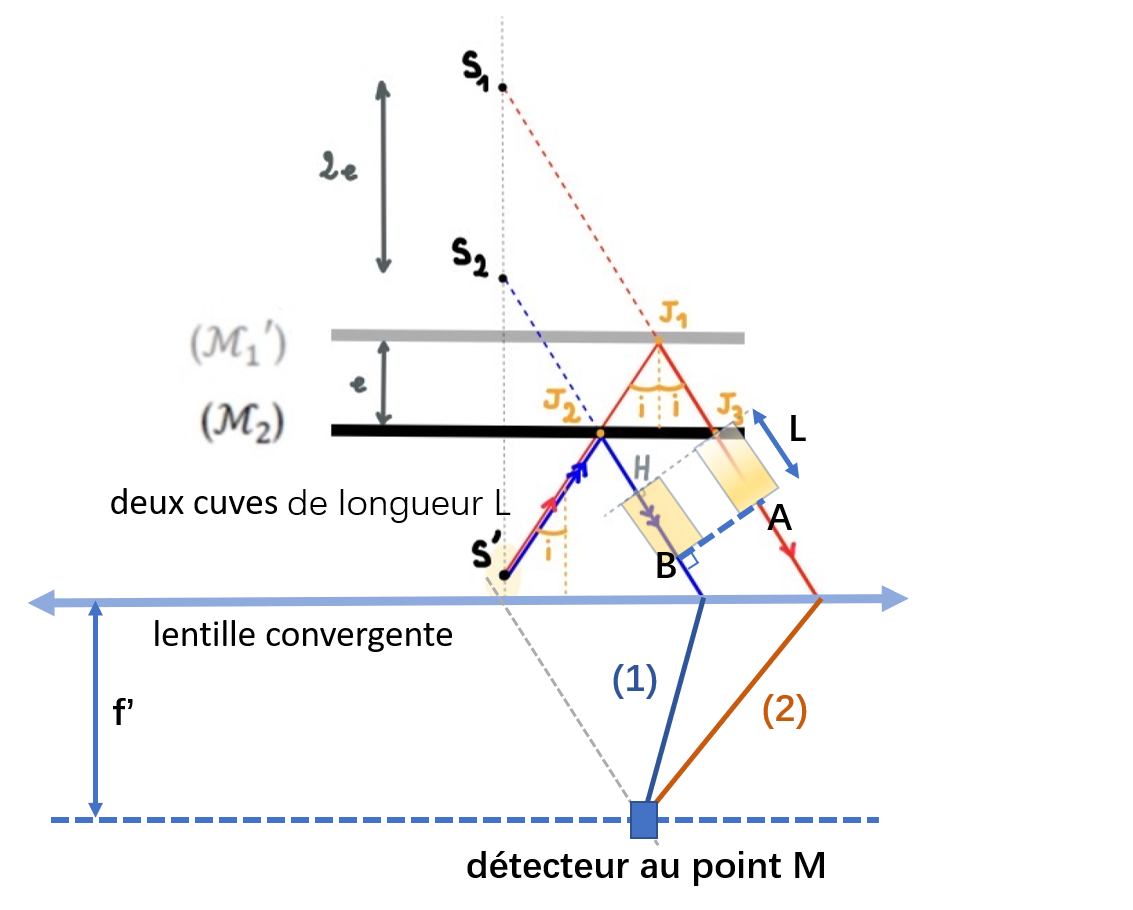
\includegraphics[scale=0.7]{tr8.png}
    \caption{Configuration de la lame d'air avec les cuves}   
\end{figure}
\begin{itemize}
    \item état initial: les deux cuves sont tous remplies d'air
          
    la différence de marche:
          \begin{align*}
            \delta_{2/1}(M)&=(S^{'}M)_2-(S^{'}M)_1\\
                           &=(S^{'}J_1J_3)+(J_3A)+(AM)-(S^{'}J_2H)-(HB)-(BM)\\
                           &=(J_2J_1J_3)-(J_2H)+(J_3A)-(HB)\\
                           &=J_2J_1J_3-J_2H+n_{air}(J_3A-HB)\\
                           &=2e\cos{i}
          \end{align*}
          comme nous avons vu en cours.

    le déphasage $\phi_{2/1}(M)=\frac{2\pi}{\lambda_0}2e\cos{i}$

    la tension détecté: $U_{i}=k*2\mathcal{E}_0\left(1+\cos \frac{2\pi}{\lambda_0}2e\cos{i}\right)$

    \item état final: il ne reste plus qu'une cuve remplie d'air
          
    la différence de marche:
          \begin{align*}
            \delta_{2/1}(M)^{'}&=(S^{'}M)_2-(S^{'}M)_1\\
                           &=(S^{'}J_1J_3)+(J_3A)+(AM)-(S^{'}J_2H)-(HB)-(BM)\\
                           &=(J_2J_1J_3)-(J_2H)+(J_3A)-(HB)\\
                           &=J_2J_1J_3-J_2H+n_{air}J_3A-HB\,\mbox{ou}\,J_2J_1J_3-J_2H+J_3A-n_{air}HB\\
                           &=2e\cos{i}\pm L(n_{air}-1)
          \end{align*}
    le déphasage $\phi_{2/1}(M)^{'}=\frac{2\pi}{\lambda_0}(2e\cos{i}\pm L(n_{air}-1))$

    la tension détecté: $U_{f}=k*2\mathcal{E}_0\left(1+\cos \frac{2\pi}{\lambda_0}(2e\cos{i}\pm L(n_{air}-1))\right)$
\end{itemize}


\begin{figure}[h]
    \centering    
    \includegraphics[scale=0.7]{Tr81.png}
    \caption{Le signal donné par le détecteur}   
\end{figure}

Pendant les deux moments, si l'on suppose que la cuve de longueur $L$ est vidée progressivement à une vitesse uniforme $l$ pendant une durée $T$. 
Pendant la transformation , la différence de marche s'écrite 

$$\delta_{2/1,T}(M)=2e\cos{i} \pm lt(1-n_{air})$$

et la tension détectée

$$U_T(t)=k*2\mathcal{E}_0\left(1+\cos\left( \left(\pm \frac{2\pi}{\lambda_0}l(n_{air}-1)\right)t+\frac{2\pi}{\lambda_0}2e\cos{i}\right)\right)$$

avec $L=lT$

Or l'enregistrement obtenu fait apparaître $N$ oscillations entre la durée $T$, la périod temporelle de $U_T(t)$ 
égale à $\frac{T}{N}$, et elle peut être aussi écrite comme $\frac{2\pi}{|\frac{2\pi}{\lambda_0}l(n_{air}-1)|}$, ce qui nous donne

$$
\frac{T}{N}=\frac{2\pi}{|\frac{2\pi}{\lambda_0}l(n_{air}-1)|}
$$
alors or $n_{air}>1$, on a 
$$
\lambda_0 N=Tl|n_{air}-1|=L(n_{air}-1)
$$
d'où $\boxed{n_{air}=1+\frac{N\lambda_0}{L}}$.

En fait, cette transformation introduit un changement d'ordre d'interférence

$$N=p_f-p_i=\frac{1}{\lambda_0}|\delta_{2/1}(M)^{'}-\delta_{2/1}(M)|=\frac{1}{\lambda_0}L(n_{air}-1)$$

ce qui nous donne le même résultat.

A.N. $n_{air}-1=\frac{46*632.8*10^{-9}}{5.0*10^{-2}}=5.8*10^{-4}$, d'où 
$\boxed{n_{air}=1.00058}$. 

L'indice de l'air est très proche de celui du vide, donc on souvent prend $n_{air}=1$ en pratique.
\end{document}